\documentclass{article}
\usepackage{tikz, comment}
\usepackage{pifont}
\usepackage{fontspec, pgfplots}
\usetikzlibrary{arrows, decorations.markings, decorations.pathreplacing}
\begin{comment}
:Title: Not defined yet
:Tags: plane figure;inverse variation, inverse proportion , inversely proportional ;direct proportion, ;focus of a parabola;truncated cone or pyramid
:Prob: 0.4692;0.4669;0.4532;0.4317;0.4284
:Author: Prof.Hu Ji-shan, HKUST
:Slug: No name yet

Description Here.........
\end{comment}
\begin{document}\centering

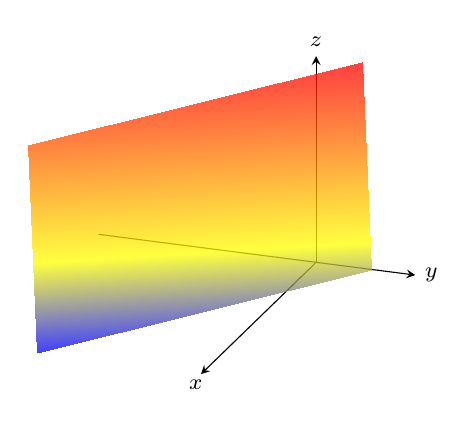
\begin{tikzpicture}[font=\footnotesize]

\begin{axis}
[axis lines = center, view={110}{30}, scale=0.8, ticks=none,
axis background, xlabel = {$x$}, ylabel ={$y$}, zlabel ={$z$}, domain =-2:2, y domain =-2:2,
samples =10, samples y =40, z buffer = auto, 
every axis x label/.style={
    at={(ticklabel* cs:1)},
    anchor= east, xshift = 4, yshift=-4
},
every axis y label/.style={
    at={(ticklabel* cs:1)},
    anchor= west, 
},
every axis z label/.style={
    at={(ticklabel* cs:1)},
    anchor= south
}]

\addplot3[surf, shader=interp, mesh/cols=2, line width = 0cm, opacity=0.75] coordinates
		{(621, -147, 206) (657, -111, 86)  (563, 31, 242) (599, 67, 122)};

\end{axis}

\end{tikzpicture}
\end{document}